\documentclass[../sherrill-Mix_thesis.tex]{subfiles}
\begin{document}
\chapter{Conclusions and future directions}
\graphicspath{{im/}{conclusion/im/}}


PacBio was bad. Figure? Do better

Comparison among labs and cell types/viruses at same time. Standardize.

Non polyadenylated RNA. Strand specific sequencing. Longer reads and longer fragments.

Ebola deaths and infected.  Ebola LAMP figure \ref{figEbolaConsensus}.

In addition an important subset of HIV are the founder viruses transmitted between hosts \citep{Keele2008,Salazar-Gonzalez2009}. These viruses are not well studied and perhaps their splicing and gene expression differ from the rest of the viral swarm of late-term patients.


\begin{figure}
	\centering
	%%[[FIX THIS FIGURE and name Ebola right]]
	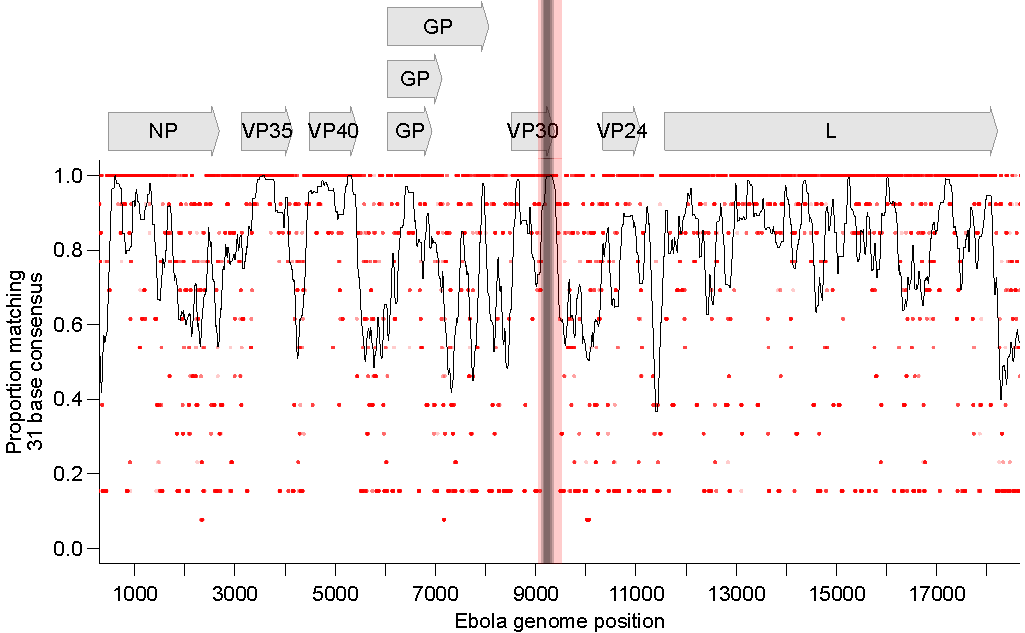
\includegraphics[width=.6\textwidth]{ebolaConsensus.pdf} %REMOVE%
	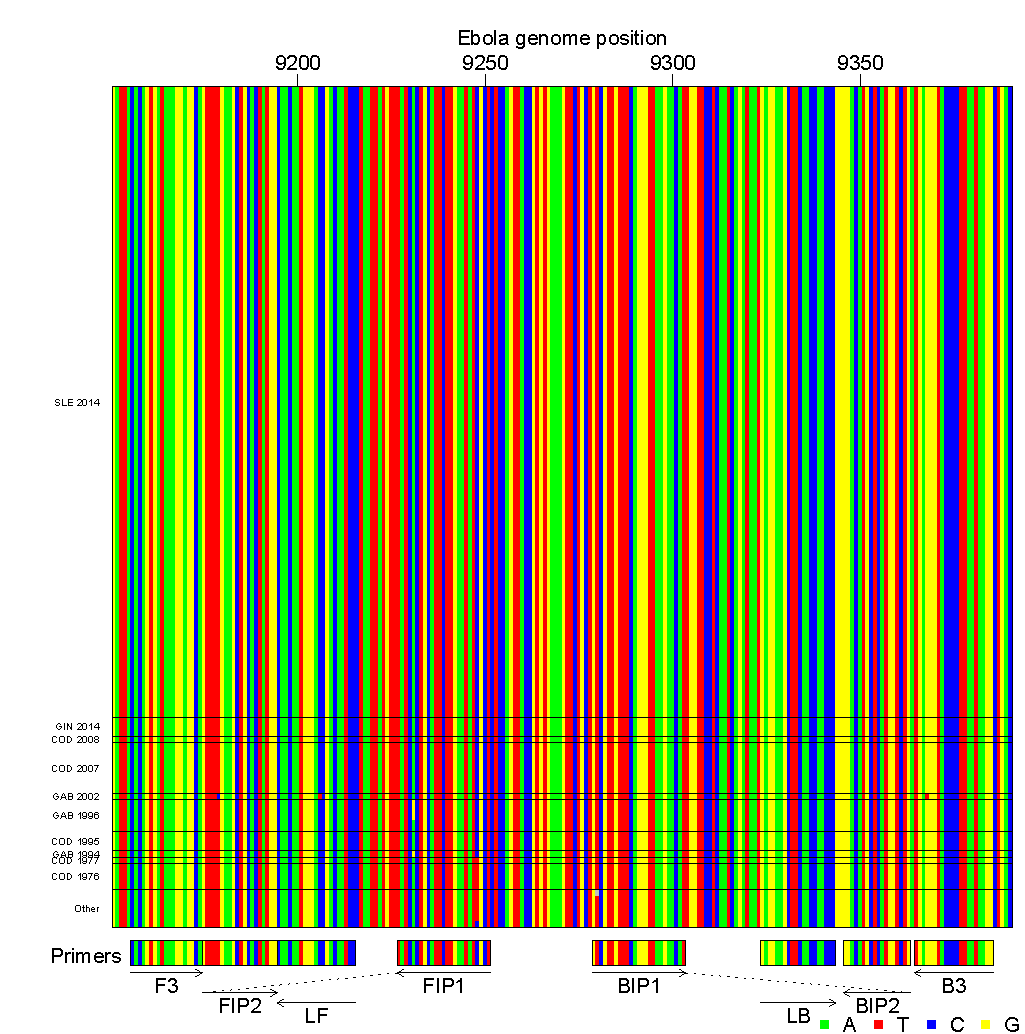
\includegraphics[width=.6\textwidth]{loop_bases.pdf} %REMOVE%
	\caption[Bioinformatic analysis to design Ebola RT-LAMP primers]{Bioinformatic analysis to design Ebola RT-LAMP primers. A) Conservation of sequence in Ebola. Ebola genomes (n = [[number]]) from the [[XXX]] collection were aligned and conservation calculated. The x-axis shows the coordinate on the Ebola genome, the y-axis shows the proportion of sequences matching the consensus for each 21 base segment of the genome (red points). The black line shows a 101 base sliding average over these proportions. The vertical red shading shows the region targeted for LAMP primer design that was used as input into the EIKEN primer design tool. Numbering is relative to the [[XX]] sequence. B) Aligned genomes, showing the locations of the preliminary primers. Sequences in the red shaded region in A are shown, with DNA bases color-coded as shown at the lower right. Each row indicates an HIV sequence and each column a base in that sequence. Horizontal lines separate the HIV subtypes (labeled at right). Arrows indicate the strand targeted by each primer. Primers targeting the negative strand of the virus are shown as reverse compliments for ease of viewing.}
	\label{figEbolaConsensus}
\end{figure}


\end{document}
